\documentclass[]{article}
\usepackage[a4paper, total={15cm,23cm}]{geometry}
\usepackage{fancyhdr}
\usepackage{graphicx}
\usepackage{amsmath}
\usepackage{amssymb}
\usepackage{xcolor}
\usepackage{tikz}
\usepackage{verbatim}
\usepackage{tcolorbox}
\usepackage{textcomp}
\usepackage{xcomment}
%opening
\title{PH 223 Week 5}
\author{Benjamin Bauml}
\date{Winter 2024}
\pagestyle{fancy}
\rhead{PH 223}
\chead{Winter 2024}
\lhead{Week 5}

% For Assignment, leave Purpose as 0. For Worksheet, set to 1. For Student Solution, set to 2. For Teacher Solution, set to 3.
\newcommand{\Purpose}{0}

\newcommand{\Exclusion}{0}
\newcommand{\PageTurn}{0}
\newcommand{\GrayProb}{0}
\newcommand{\Tipsy}{0}

% Assignment
\if\Purpose0
\renewcommand{\Exclusion}{1}
\fi
% Worksheet
\if\Purpose1
\renewcommand{\Exclusion}{1}
\renewcommand{\PageTurn}{1}
\fi
% Student Solution
\if\Purpose2
\renewcommand{\PageTurn}{1}
\renewcommand{\GrayProb}{1}
\fi
% Teaching Copy
\if\Purpose3
\renewcommand{\PageTurn}{1}
\renewcommand{\GrayProb}{1}
\renewcommand{\Tipsy}{1}
\fi

\if\Exclusion1
\xcomment{Title,Problem,ProblemSub,PassFig}
\fi

\def \NewQ {0}
\newcommand{\MaybePage}{
	\if\NewQ0
	\gdef \NewQ {\PageTurn}
	\else
	\newpage
	\fi
}

\newenvironment{Problem}[1]{
\MaybePage
\section*{#1}
\if\GrayProb1
\begin{tcolorbox}[colback=lightgray,colframe=lightgray,sharp corners,boxsep=1pt,left=0pt,right=0pt,top=0pt,bottom=0pt,after skip=2pt]
\else
\begin{tcolorbox}[colback=white,colframe=white,sharp corners,boxsep=1pt,left=0pt,right=0pt,top=0pt,bottom=0pt,after skip=2pt]
\fi
}{
\end{tcolorbox}\noindent
}

\newenvironment{ProblemSub}{
\if\GrayProb1
\begin{tcolorbox}[colback=lightgray,colframe=lightgray,sharp corners,boxsep=1pt,left=0pt,right=0pt,top=0pt,bottom=0pt,after skip=2pt]
\else
\begin{tcolorbox}[colback=white,colframe=white,sharp corners,boxsep=1pt,left=0pt,right=0pt,top=0pt,bottom=0pt,after skip=2pt]
\fi
}{
\end{tcolorbox}\noindent
}

\newenvironment{PassFig}{\begin{figure}[h]}{\end{figure}}

\newcommand{\TeachingTips}[1]{
\if\Tipsy1
\begin{tcolorbox}[colback=lightgray,colframe=black]
#1
\end{tcolorbox}
\fi
}

\newenvironment{Title}{\maketitle}{}

\begin{document}
\begin{Title}
\begin{center}
	These problems are borrowed/adapted from \textit{Physics for Scientists and Engineers}, the first two from Chapter 26, and the third from Chapter 22.
\end{center}
\end{Title}

\begin{Problem}{Activity 1}
	(a) How much work does the charge escalator do to move 1.0 \textmu C of charge from the negative terminal to the positive terminal of a 1.5 V battery?
\end{Problem}
The work done is equal to the increase in the potential energy of the charge:
\[
W = \Delta U = q\Delta V = (1.0\times10^{-6}\text{ C})(1.5\text{ V}) = 1.5\times10^{-6}\text{ J}.
\]
The charge escalator does 1.5 \textmu J of work.
\begin{ProblemSub}
	(b) How much charge does a 9.0 V battery transfer from the negative to the positive terminal while doing 27 J of work?
\end{ProblemSub}
As before, $ W = q\Delta V $, so solving for charge gets us
\[
q = \frac{W}{\Delta V} = \frac{27\text{ J}}{9.0\text{ V}} = 3.0\text{ C}.
\]
The battery transfers 3.0 C of charge.
\begin{ProblemSub}
	(c) Light from the sun allows a solar cell to move electrons from the positive to the negative terminal, doing $ 2.4\times10^{-19} $ J of work per electron. What is the emf of this solar cell?
\end{ProblemSub}
Knowing that emf is intimately related to potential difference, let us begin with the fact that $ W = q\Delta V = -e\Delta V $ for moving an electron from the positive terminal to the negative terminal. Solving for $ \Delta V $, we get
\[
\Delta V = \frac{W}{-e} = \frac{2.4\times10^{-19}\text{ J}}{-1.6\times10^{-19}\text{ C}} = -1.5\text{ V}.
\]
The potential difference from the positive to the negative terminal is $ -1.5 $ V, but our charge escalator model has emf work to move positive charge from the negative terminal to the positive terminal, so $ \mathcal{E} = 1.5 $ V.
\TeachingTips{
Students may need to be reminded that work is equal to the change in potential energy in this context.

We do not use electromotive force in this course, so tell students just to think of it as $\Delta V$. Since it isn't a force, the terms \textit{source voltage} or \textit{source tension} (the latter of which seems equally stupid) are now favored by certain international standards organizations (according to Wikipedia). It is an energy per unit charge provided to a circuit by a transducer---that being any device which converts energy (such as chemical energy for a battery, or mechanical energy for a generator) to electrical energy.
}

\begin{Problem}{Activity 2}
	You need to construct a 100 pF capacitor for a science project. You plan to cut two $ L\times L $ metal squares and insert small spacers between their corners. The thinnest spacers you have are 0.20 mm thick. What is the proper value of $ L $?
\end{Problem}
We know $ A = L^{2} $ for the parallel-plate capacitor we are making, so
\[
C = \frac{\epsilon_{0}L^{2}}{d} \implies L = \sqrt{\frac{Cd}{\epsilon_{0}}} = \sqrt{\frac{(1.00\times10^{-10}\text{ F})(2.0\times10^{-4}\text{ m})}{8.85\times10^{-12}\text{ C}^{2}/\text{N m}^{2}}} \approx 0.048\text{ m}.
\]
The plates must have a side length of $ 4.8 $ cm. Note that 1 F is equal to 1 C/V, which is 1 C$ ^{2} $/J, so the units in the radicand work out to meters squared.
\TeachingTips{
If students have trouble starting, they should have seen the electric field between charged parallel plates of area $A$:
\[
E = \frac{Q}{\epsilon_{0} A}.
\]
For plate separation $d$, this gives the potential difference
\[
\Delta V = \frac{Qd}{\epsilon_{0} A}.
\]
Capacitance is charge divided by potential difference (ergo one farad is equal to one coulomb per volt), so we find
\[
C = \frac{Q}{\Delta V} = \frac{\epsilon_{0}A}{d}.
\]
}

\begin{Problem}{Activity 3}
	Two neutral metal spheres on wood stands are touching. A negatively charged rod is held directly above the top of the left sphere, not quite touching it. While the rod is there, the right sphere is moved so that the spheres no longer touch. Then the rod is withdrawn. Afterward, what is the charge state of each sphere? Use charge diagrams to explain your answer.
\end{Problem}
\begin{center}
	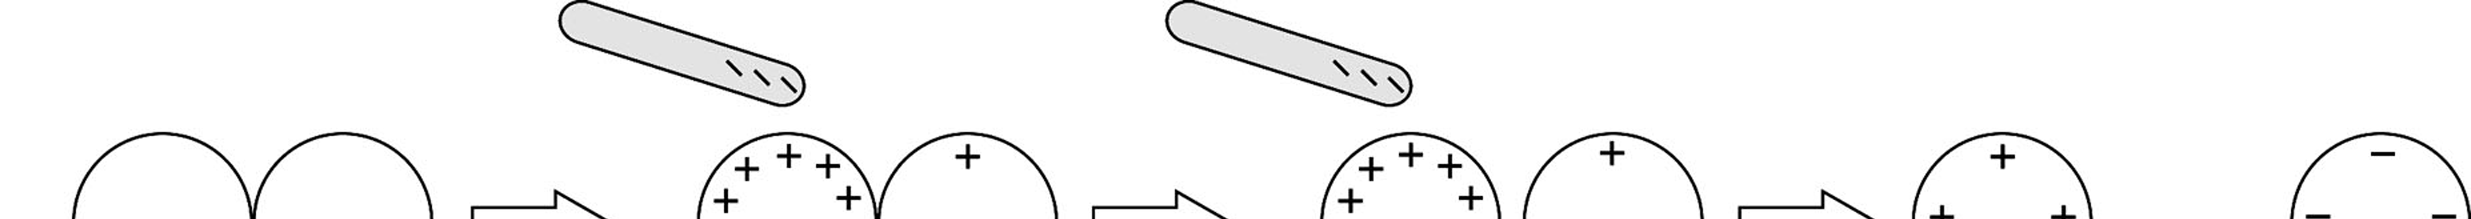
\includegraphics[scale=0.1]{SpheryHorror}\vspace{-0.5pt}
	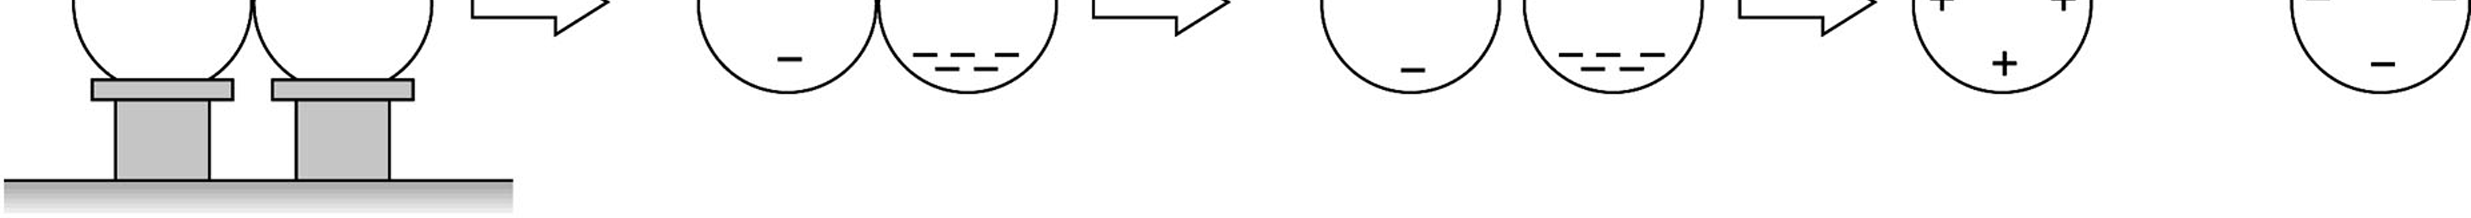
\includegraphics[scale=0.1]{SpheryHorrorLowerHalf}
\end{center}
\begin{itemize}
	\item The first step shows two neutral metal spheres touching each other.
	\item In the second step, the negative rod repels the negative charges, which will retreat as far as possible from the top of the left sphere. Note that the two spheres are touching and the net charge on these two spheres is still zero.
	\item While the rod is there on top of the left sphere, the right sphere is moved away from the left sphere. Because the right sphere has an excess negative charge, charge conservation implies the left sphere must have the same magnitude of positive charge. Upon separation, the negative charge is trapped on the right sphere, as shown in the third step.
	\item As the two spheres are moved farther apart and the negatively charged rod is moved away from the spheres, the charges on the two spheres redistribute uniformly over the entire surface of each sphere. Thus, we are left with two oppositely charged spheres.
\end{itemize}
\end{document}
